\documentclass[12pt,letterpaper]{article}

%Packages
\usepackage{pdflscape}
\usepackage{fixltx2e}
\usepackage{textcomp}
\usepackage{fullpage}
\usepackage{natbib}
\usepackage{float}
\usepackage{latexsym}
\usepackage{url}
\usepackage{epsfig}
\usepackage{graphicx}
\usepackage{amssymb}
\usepackage{amsmath}
\usepackage{bm}
\usepackage{array}
\usepackage[version=3]{mhchem}
\usepackage{ifthen}
\usepackage{caption}
\usepackage{hyperref}
\usepackage{amsthm}
\usepackage{amstext}
\usepackage{enumerate}
\usepackage[osf]{mathpazo}
\usepackage{dcolumn}
\usepackage{lineno}
\pagenumbering{arabic}

%Pagination style and stuff
\linespread{2}
\raggedright
\setlength{\parindent}{0.5in}
\setcounter{secnumdepth}{0} 
\renewcommand{\section}[1]{%
\bigskip
\begin{center}
\begin{Large}
\normalfont\scshape #1
\medskip
\end{Large}
\end{center}}
\renewcommand{\subsection}[1]{%
\bigskip
\begin{center}
\begin{large}
\normalfont\itshape #1
\end{large}
\end{center}}
\renewcommand{\subsubsection}[1]{%
\vspace{2ex}
\noindent
\textit{#1.}---}
\renewcommand{\tableofcontents}{}
\bibpunct{(}{)}{;}{a}{}{,}

\begin{document}

\section{Code}
All code for performing the analyses is available at: \url{https://github.com/TGuillerme/Total_Evidence_Method-Missing_data}.

\newpage
\section{Appendix 1: Tree Building}
  \section{Supplementary material Section 1}

\subsection{Morphological characters states}
In order to obtain a realistic probabilistic value for of \textit{k} characters states for each simulated morphological character, we downloaded 100 random morphological characters (with more than 100 characters each) from TreeBASE database (http://treebase.org/) published between 1985 and 2013 and covering 19 taxomomic classess (Chordata, Arthropoda, Annelida, Angiosperm, Gymnosperm and Pteridophyta).
We selected a total of 22563 characters ranging from 2 to 10 states.
We calculated the proportion of characters with 2, 3, 4, 5, 6, 7, 8, 9 or 10 states.
We then sampeled 22563 \textit{k} values between 2 and 10 with the same proportion of characters from the empirical data.
We then used a simple t-test to check if our simulation was equal to the empirical data.
In this study, we only simulated characters with 2 or 3 states because of the high proportion of ordered characters ecountered on characters with more than 3 states and the difficulties of simulate biologicaly sensible ordered characters.

\begin{figure}
\centering
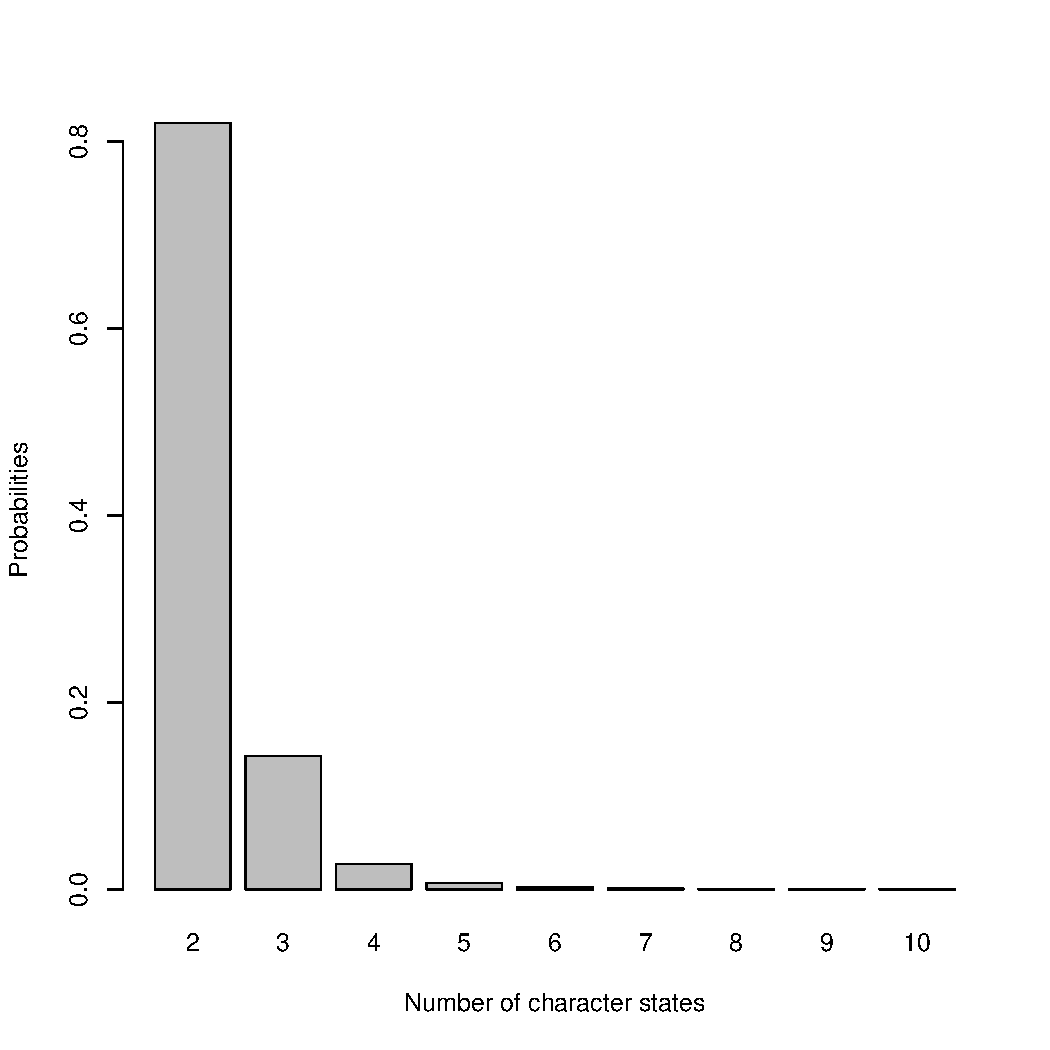
\includegraphics[keepaspectratio=true]{Figures/Supplementary/TEM_Fig-AppendixCharacters.pdf}
\caption{Character states distribution in empirical matrices. %Title?
Characters states number distribution extracted from 100 random morphological matrices downloaded from RreeBase.}
\label{Fig_AppendixCharacters}
\end{figure}


\subsection{Tree Building Software settings}

\subsubsection{Maximum Likelihood - RAxML v8.0.20 \citep{Stamatakis21012014}}

Model: \\
Molecular data: \\
GTR + $\Gamma_4$ (-m GTRGAMMA) \\
Morphological data: \\
Mk + $\Gamma_4$ (-K MK) \\
Support: \\
Rapid Boostrap algorithm (LSR), 1000 replicates \\

\subsubsection{Bayesian - MrBayes v3.2.1 \citep{Ronquist2012mrbayes}}

Priors: \\
Molecular data: \\
rates distribution shape ($\alpha$) = 0.5 \\
Transition/Transversion ratio = 2 ($\beta$(80,40)) \\
Starting tree: "True" tree topology with each branch length = 1 \\
Morphological data: \\
rates distribution shape ($\alpha$) = 0.5 \\
Models: \\
Molecular data: HKY + $\Gamma_4$ \\
Morphological data: Mk + $\Gamma_4$ \\
MCMC: \\
2 runs \\
4 chains per run \\
generations < 50$\times$$1^6$ \\
sample frequency = 1050$\times$$1^3$ \\
ASDS diagnosis frequency = 50$\times$$1^3$ \\
ASDS $<$ 0.01 \\
ESS $>>$ 200 \\
Burnin = 25\%
  \label{Supp_TreeBuilding}

\newpage
\section{Appendix 2: Tree Comparisons}
  %\section{Supplementary material Section 2}

\subsection{Robinson-Foulds distance}
Robinson-Foulds distance (\textit{RF}; \citealp{RF1981}), or "path difference", measures the number of shared clades across two trees. The metric reflects the distance between the distributions of tips among clades in the two trees \citep{RF1981} and can be expressed as:
\begin{equation}
RF_{x,y} = N_{x} + N_{y} - 2C_{x,y}
\end{equation}
where $C_{x,y}$ is the number of clades in common in the two trees. $C$ is equal to one if the two trees have the same $n$ taxa; and $C = n-2$ when none of the $n$ taxa are shared between the trees. This metric is more sensitive to taxon displacement than Triplets distance (i.e. if one taxon moves out of a clade, then the clades are no longer considered similar; \citet{critchlowthe1996,johnson1998,wiensmissing2003}). The minimal value of $C$ is equal to 1 if the two trees have the same n taxa; the maximal value in $C = n-2$. For a fully unresolved tree (star tree) $N$=1 and for a fully resolved tree (binary tree) $N = n-2$. The minimal and maximal topological distance for taxa is:
\begin{equation}
RF_{min} = 1 + 1 - 2C_{x,y}
\end{equation}
and:
\begin{equation}
RF_{max} = 2(n-2)-2
\end{equation}
One can then rescale \textit{RF.scaled} by using the maximal and minimal value for any $n$ taxa:
\begin{equation}
RF.scaled_{x,y} = \frac{RF_{x,y}-RF_{max}}{RF_{max}}
\end{equation}
This metric is more sensitive to taxa displacement than the Triplets distance \citep{critchlowthe1996,johnson1998,wiensmissing2003} and therefore a low value will show a good clade conservation between two trees and a high value will show a bad recovery of common clades.

\subsection{Triplets distance details ($T_{x,y}$)}
Triplets distance ($T_{x,y}$; \citealp{dobson1975triplets}) measures the number of sub-trees made up of three taxa (triplets) that differ between two given trees. Each triplet can be written as $I_{ijk}$=(\textit{ijk}). Where $I_{ijk}$ is equal to zero if the the two triplets (\textit{ijk}) are the same in the two trees otherwise $I_{ijk}$ is equal to one. For any rooted binary tree there are only three possible combinations for each triplet: ((\textit{j},\textit{k}),\textit{i});, ((\textit{i},\textit{k}),\textit{j}); and ((\textit{i},\textit{j}),\textit{k}); \citep{johnson1998}. If the trees used are not fully binary, a fourth triplet combination is possible: (\textit{i},\textit{j},\textit{k}). We can calculate the triplet distance between two trees, $S_n$, as:
\begin{equation}
S_n = \sum_{ijk} I_{ijk}
\end{equation}
where:
\begin{equation}
\sum_{ijk} = \binom{n}{4} = \frac{n!}{4!(n-4)!}
\end{equation}
and where \textit{n} is the total number of taxa in both trees (modified from \citet{critchlowthe1996}). If $S_n$ = 0, the trees are identical; when $S_n$ = $\binom{n}{4}$, the trees are as different as possible (i.e. every taxon has a different placement in the two trees). Because the possible number of triplets per clade is a finite number, the probability of two random trees with the same $n$ taxa to have the same triplet is:
\begin{equation}
P({I_{ijk}}=0) = \frac{1}{4}
\end{equation}
Therefore one can calculate the probability of two random trees having the same triplets: 
\begin{equation}
P({S_{n}}=0) = \sum_{ijk} P_{I_{ijk}=0}
\end{equation}
\begin{equation}
P({S_{n}}=0) = \frac{n!}{4(3!(n-3)!}
\end{equation}
and in the same way:
\begin{equation}
P({S_{n}}=1) = \frac{3n!}{4(3!(n-3)!}
\end{equation}

\subsection{Normalised Tree Similarity}
For any tree with \textit{n} taxa compared using a tree distance metric $m$, Normalized Tree Similarity, $NTS_m$ \citep{Bogdanowicz2012}, represents the similarity score for the two trees given the expected distance between two random Yule trees with $n$ taxa. If $\bar{d}_{m,n}$\textit{(rand)} is the average distance between two random Yule trees with $n$ taxa and $d_{m,n}$\textit{(x,y)} the distance between the two trees \textit{x} and \textit{y} each containing $n$ taxa, then:
\begin{equation}
NTS_{m,n}(x,y)=\frac{\bar{d}_{m,n}(rand) - d_{m,n}(x,y)} {\bar{d}_{m,n}(rand)}
\end{equation}
\textit{NTS} ranges from one to -$\infty$.
For any $m,n$, when $NTS$ = 1, the trees are identical, when \textit{NTS} = 0 the trees are no more different than expected by chance, and when $NTS$ $<$ 0, the trees are more different than expected when comparing two random trees. 

We used the NTS method to scale all the Robinson Foulds and Triplets distances calculated in our analyses, using the TreeCmp java script \citep{Bogdanowicz2012}.

\subsection{Bhattacharyya Coefficient}
The Bhattacharyya Coefficient calculates the probability of overlap of two distributions \citep{Bhattacharyya}. When it is equal to zero, the probability of overlap of the distributions is also zero, and when it is equal to one, the two distributions are entirely overlapping. It forms an elegant and easy to compute continuous measurement of the probability of similarity between two distributions. The coefficient is calculated as the sum of the square root of the relative counts shared in \textit{n} bins among two distributions.
\begin{equation}
\text{Bhattacharyya Coefficient}=\sum_{i=1}^{n} \sqrt{{\sum{a_i}}\times{\sum{b_i}}}
\end{equation}
where
\begin{equation}
\sum{a_i}=\frac{\text{Number of counts in bin \textit{i} for the distribution \textit{a}}}{\text{Total number of counts for the distribution \textit{a}}}
\end{equation}
and
\begin{equation}
\sum{b_i}=\frac{\text{Number of counts in bin \textit{i} for the distribution \textit{b}}}{\text{Total number of counts for the distribution \textit{b}}}
\end{equation}
The precision of the Bhattacharyya Coefficient is directly related to the number of bins, $n$. If $n$ is low, the overlap will be overestimated and if $n$ is too high, the overlap will be underestimated. In this analysis, we determined the number of bins using Silverman's rule of thumb which states that $n$ should be 0.9 times the minimum of the standard deviation and the interquartile range of the distribution, divided by 1.34 times the sample size of the distribution to the negative one-fifth power (bw.nrd0() function in R; \citet{silverman1986density}).

  \label{Supp_TreeComparison}

\bibliographystyle{sysbio}
\bibliography{Supp_Ref}

\newpage
\section{Appendix 3: Additional Results}
  \section{Supplementary material Section 3}

\begin{figure} 
\centering
    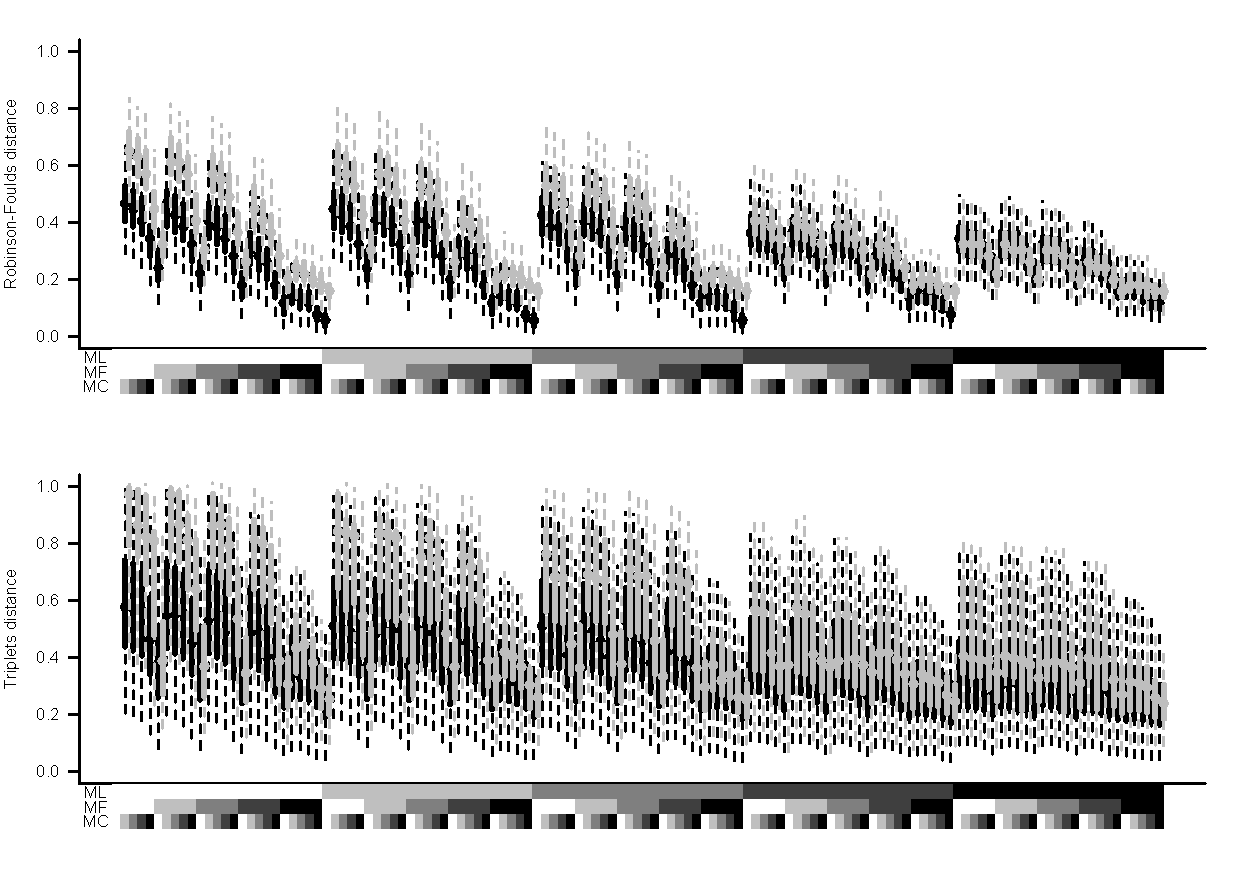
\includegraphics[width=1\textwidth]{SupplementaryMaterial/Supp_Figures/Boot+Baytre-AllParam-RF+Tr.pdf}
\caption{Trend of the effect of missing data on topological recovery on the Bootstraps and the Bayesian posterior trees distributions. The amount of missing data per parameter ($M_{L}$, $M_{F}$ and $M_{C}$) is represented along the x axis. The colour gradient from white to black represents respectively, 0\%, 10\%, 25\%, 50\% and 75\% of missing data. The topological recovery is represented on the y axis, both using Robinson-Foulds distance (upper row) and Triplets distance (lower row). Points represent the modal value of each distribution ; thick solid and thin dashed lines represents respectively the 50\% and 95\% confidence intervals or the distributions. The Bootstraps are represented in black and the Bayesian posterior trees distributions in grey.}
\label{Fig_global_BootTreesets} %Differences between all the parameters and between two methods (Boot vs treesets)
\end{figure}

\begin{figure} 
\centering
    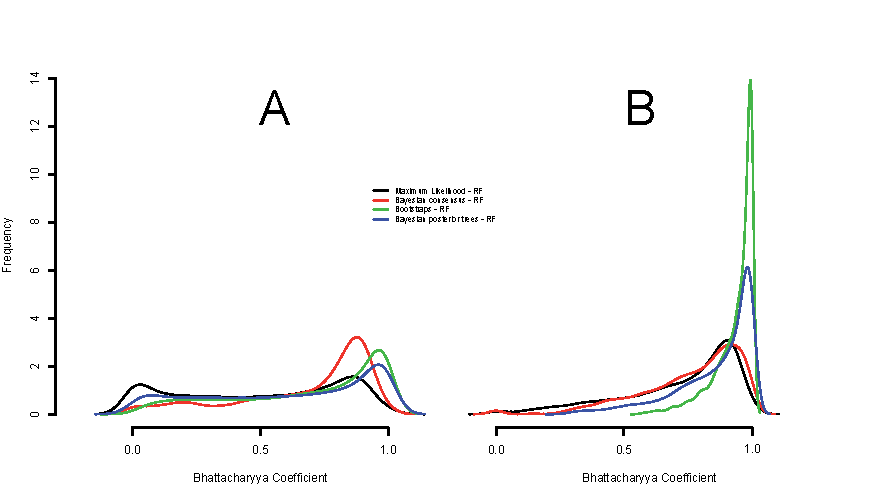
\includegraphics[width=1\textwidth]{SupplementaryMaterial/Supp_Figures/BC-AllMethods-RF+Tr.pdf}
\caption{Distribution of the Pairwise Bhattacharyya Coefficients within each method. A- Distribution of the coefficients when comparing Ronbinson-Foulds distances. B- Distribution of the coefficients when comparing Triplets distances.}
\label{Fig_Bhatt.coeff_distribution} %Differences in overlap within each method
\end{figure}

\begin{figure} 
\centering
    \includegraphics[width=1\textwidth]{SupplementaryMaterial/Supp_Figures/PairwiseComp-ML-RF+Tr.pdf}
\caption{Pairwise Bhattacharyya Coefficients within the Maximum Likelihood trees. The pairwise trees comparisons are represent on both axis. The colour gradient from white to black represents respectively, 0\%, 10\%, 25\%, 50\% and 75\% of missing data for each parameter. The matrix represents the values of pairwise Bhattacharyya Coefficients going from green (1) to red (0). A. Results for the Normalised Robinson-Foulds distance. B. Results with the for Normalised Triplets distance.}
\label{Fig_pairComp-Baytree-RF}
\end{figure} %Pairwise BC for the ML for RF+Tr. (parameters differences)

\begin{figure} 
\centering
    \includegraphics[width=1\textwidth]{SupplementaryMaterial/Supp_Figures/PairwiseComp-Boot-RF+Tr.pdf}
\caption{Pairwise Bhattacharyya Coefficients within the Bootstrap trees. The pairwise trees comparisons are represent on both axis. The colour gradient from white to black represents respectively, 0\%, 10\%, 25\%, 50\% and 75\% of missing data for each parameter. The matrix represents the values of pairwise Bhattacharyya Coefficients going from green (1) to red (0). A. Results for the Normalised Robinson-Foulds distance. B. Results with the for Normalised Triplets distance.}
\label{Fig_pairComp-Baytree-Tr}
\end{figure} %Pairwise BC for the Boot for RF+Tr. (parameters differences)

\begin{figure} 
\centering
    \includegraphics[width=1\textwidth]{SupplementaryMaterial/Supp_Figures/PairwiseComp-Baytre-RF+Tr.pdf}
\caption{Pairwise Bhattacharyya Coefficients within the Bayesian posterior distribution trees. The pairwise trees comparisons are represent on both axis. The colour gradient from white to black represents respectively, 0\%, 10\%, 25\%, 50\% and 75\% of missing data for each parameter. The matrix represents the values of pairwise Bhattacharyya Coefficients going from green (1) to red (0). A. Results for the Normalised Robinson-Foulds distance. B. Results with the for Normalised Triplets distance.}
\label{Fig_pairComp-MLbest-RF}
\end{figure} %Pairwise BC for the Baytre for RF+Tr. (parameters differences)


%Summary of metrics values for all parameters combinations
\begin{table}[ht]
\centering
\begin{tabular}{rrrrrrr}
  \hline
 & Min. & 1st Qu. & Median & Mean & 3rd Qu. & Max. \\ 
  \hline
  Maximum likelihood-RF & 0.06 & 0.26 & 0.40 & 0.41 & 0.50 & 0.95 \\ 
  Maximumlikelihood-Tr & 0.29 & 0.45 & 0.59 & 0.63 & 0.84 & 1.00 \\ 
  Bayesian consensus-RF & 0.69 & 0.71 & 0.72 & 0.76 & 0.79 & 0.96 \\ 
  Bayesian consensus-Tr & -0.28 & -0.11 & 0.17 & 0.19 & 0.37 & 0.98 \\ 
  Bootstraps-RF & 0.06 & 0.18 & 0.27 & 0.26 & 0.34 & 0.46 \\ 
  Bootstraps-Tr & 0.23 & 0.31 & 0.35 & 0.38 & 0.45 & 0.58 \\ 
  Bayesian posterior trees-RF & 0.16 & 0.22 & 0.32 & 0.34 & 0.42 & 0.65 \\ 
  Bayesian posterior trees-Tr & 0.24 & 0.35 & 0.40 & 0.50 & 0.67 & 0.98 \\ 
   \hline
   \hline
\end{tabular}
\end{table}

%Summary of metrics values for the ML parameter
\begin{table}[ht]
\centering
\begin{tabular}{rrrrrrr}
  \hline
 & Min. & 1st Qu. & Median & Mean & 3rd Qu. & Max. \\ 
  \hline
Maximum likelihood-RF & 0.44 & 0.51 & 0.63 & 0.66 & 0.78 & 0.95 \\ 
  Maximumlikelihood-Tr & 0.45 & 0.56 & 0.76 & 0.74 & 0.93 & 0.99 \\ 
  Bayesian consensus-RF & 0.71 & 0.73 & 0.80 & 0.82 & 0.88 & 0.95 \\ 
  Bayesian consensus-Tr & 0.37 & 0.46 & 0.67 & 0.67 & 0.87 & 0.96 \\ 
  Bootstraps-RF & 0.34 & 0.37 & 0.42 & 0.41 & 0.44 & 0.46 \\ 
  Bootstraps-Tr & 0.32 & 0.40 & 0.51 & 0.46 & 0.51 & 0.57 \\ 
  Bayesian posterior trees-RF & 0.33 & 0.41 & 0.52 & 0.50 & 0.60 & 0.65 \\ 
  Bayesian posterior trees-Tr & 0.41 & 0.56 & 0.76 & 0.71 & 0.84 & 0.98 \\ 
   \hline
\end{tabular}
\end{table}

%Summary of metrics values for the ML parameter
\begin{table}[ht]
\centering
\begin{tabular}{rrrrrrr}
  \hline
 & Min. & 1st Qu. & Median & Mean & 3rd Qu. & Max. \\ 
  \hline
Maximum likelihood-RF & 0.23 & 0.46 & 0.64 & 0.61 & 0.79 & 0.93 \\ 
  Maximumlikelihood-Tr & 0.65 & 0.84 & 0.95 & 0.89 & 0.99 & 1.00 \\ 
  Bayesian consensus-RF & 0.72 & 0.77 & 0.86 & 0.85 & 0.94 & 0.96 \\ 
  Bayesian consensus-Tr & -0.16 & 0.19 & 0.63 & 0.52 & 0.96 & 0.98 \\ 
  Bootstraps-RF & 0.14 & 0.30 & 0.40 & 0.35 & 0.45 & 0.46 \\ 
  Bootstraps-Tr & 0.37 & 0.49 & 0.54 & 0.51 & 0.56 & 0.57 \\ 
  Bayesian posterior trees-RF & 0.24 & 0.45 & 0.57 & 0.51 & 0.63 & 0.65 \\ 
  Bayesian posterior trees-Tr & 0.44 & 0.81 & 0.86 & 0.82 & 0.98 & 0.98 \\ 
   \hline
\end{tabular}
\end{table}

%Summary of metrics values for the MC parameter
\begin{table}[ht]
\centering
\begin{tabular}{rrrrrrr}
  \hline
 & Min. & 1st Qu. & Median & Mean & 3rd Qu. & Max. \\ 
  \hline
Maximum likelihood-RF & 0.40 & 0.50 & 0.64 & 0.65 & 0.79 & 0.94 \\ 
  Maximumlikelihood-Tr & 0.70 & 0.84 & 0.93 & 0.89 & 0.99 & 1.00 \\ 
  Bayesian consensus-RF & 0.76 & 0.79 & 0.86 & 0.86 & 0.92 & 0.96 \\ 
  Bayesian consensus-Tr & 0.05 & 0.16 & 0.53 & 0.50 & 0.87 & 0.92 \\ 
  Bootstraps-RF & 0.25 & 0.34 & 0.42 & 0.38 & 0.45 & 0.46 \\ 
  Bootstraps-Tr & 0.38 & 0.47 & 0.55 & 0.51 & 0.57 & 0.58 \\ 
  Bayesian posterior trees-RF & 0.32 & 0.44 & 0.58 & 0.52 & 0.62 & 0.65 \\ 
  Bayesian posterior trees-Tr & 0.39 & 0.78 & 0.82 & 0.79 & 0.98 & 0.98 \\ 
   \hline
\end{tabular}
\end{table}


%Summary of the BC between pairs of methods for the ML parameter
\begin{table}[ht]
\centering
\begin{tabular}{rrrrrrr}
  \hline
 & Min. & 1st Qu. & Median & Mean & 3rd Qu. & Max. \\ 
  \hline
Maximum.likelihood.vs..Bayesian.consensus...RF & 0.30 & 0.31 & 0.69 & 0.61 & 0.77 & 1.00 \\ 
  Maximum.likelihood.vs..Bayesian.consensus...Tr & 0.79 & 0.81 & 0.84 & 0.86 & 0.85 & 1.00 \\ 
  Maximum.likelihood.vs..Bootstraps...RF & 0.03 & 0.22 & 0.29 & 0.36 & 0.54 & 0.69 \\ 
  Maximum.likelihood.vs..Bootstraps...Tr & 0.08 & 0.42 & 0.53 & 0.51 & 0.74 & 0.78 \\ 
  Maximum.likelihood.vs..Bayesian.posterior.trees...RF & 0.02 & 0.49 & 0.61 & 0.51 & 0.67 & 0.74 \\ 
  Maximum.likelihood.vs..Bayesian.posterior.trees...Tr & 0.21 & 0.61 & 0.70 & 0.63 & 0.81 & 0.81 \\ 
  Bayesian.consensus.vs..Bootstraps...RF & 0.01 & 0.02 & 0.02 & 0.02 & 0.03 & 0.04 \\ 
  Bayesian.consensus.vs..Bootstraps...Tr & 0.08 & 0.69 & 0.78 & 0.64 & 0.79 & 0.84 \\ 
  Bayesian.consensus.vs..Bayesian.posterior.trees...RF & 0.01 & 0.02 & 0.02 & 0.04 & 0.08 & 0.09 \\ 
  Bayesian.consensus.vs..Bayesian.posterior.trees...Tr & 0.21 & 0.74 & 0.75 & 0.68 & 0.84 & 0.87 \\ 
  Boostraps.vs..Bayesian.posterior.trees...RF & 0.69 & 0.75 & 0.85 & 0.85 & 0.95 & 1.00 \\ 
  Boostraps.vs..Bayesian.posterior.trees...Tr & 0.91 & 0.92 & 0.96 & 0.95 & 0.97 & 0.98 \\ 
   \hline
\end{tabular}
\end{table}

%Summary of the BC between pairs of methods for the MF parameter
\begin{table}[ht]
\centering
\begin{tabular}{rrrrrrr}
  \hline
 & Min. & 1st Qu. & Median & Mean & 3rd Qu. & Max. \\ 
  \hline
Maximum.likelihood.vs..Bayesian.consensus...RF & 0.00 & 0.25 & 0.48 & 0.50 & 0.76 & 1.00 \\ 
  Maximum.likelihood.vs..Bayesian.consensus...Tr & 0.38 & 0.69 & 0.75 & 0.72 & 0.80 & 1.00 \\ 
  Maximum.likelihood.vs..Bootstraps...RF & 0.03 & 0.18 & 0.32 & 0.36 & 0.47 & 0.77 \\ 
  Maximum.likelihood.vs..Bootstraps...Tr & 0.08 & 0.34 & 0.40 & 0.38 & 0.53 & 0.55 \\ 
  Maximum.likelihood.vs..Bayesian.posterior.trees...RF & 0.02 & 0.47 & 0.71 & 0.60 & 0.86 & 0.94 \\ 
  Maximum.likelihood.vs..Bayesian.posterior.trees...Tr & 0.21 & 0.54 & 0.62 & 0.56 & 0.64 & 0.80 \\ 
  Bayesian.consensus.vs..Bootstraps...RF & 0.00 & 0.00 & 0.01 & 0.01 & 0.01 & 0.03 \\ 
  Bayesian.consensus.vs..Bootstraps...Tr & 0.08 & 0.38 & 0.54 & 0.49 & 0.70 & 0.75 \\ 
  Bayesian.consensus.vs..Bayesian.posterior.trees...RF & 0.00 & 0.02 & 0.02 & 0.02 & 0.04 & 0.04 \\ 
  Bayesian.consensus.vs..Bayesian.posterior.trees...Tr & 0.21 & 0.29 & 0.66 & 0.54 & 0.72 & 0.82 \\ 
  Boostraps.vs..Bayesian.posterior.trees...RF & 0.69 & 0.69 & 0.72 & 0.71 & 0.72 & 0.72 \\ 
  Boostraps.vs..Bayesian.posterior.trees...Tr & 0.91 & 0.91 & 0.91 & 0.93 & 0.92 & 0.98 \\ 
   \hline
\end{tabular}
\end{table}

%Summary of the BC between pairs of methods for the MC parameter
\begin{table}[ht]
\centering
\begin{tabular}{rrrrrrr}
  \hline
 & Min. & 1st Qu. & Median & Mean & 3rd Qu. & Max. \\ 
  \hline
Maximum.likelihood.vs..Bayesian.consensus...RF & 0.03 & 0.32 & 0.66 & 0.55 & 0.75 & 1.00 \\ 
  Maximum.likelihood.vs..Bayesian.consensus...Tr & 0.51 & 0.69 & 0.80 & 0.76 & 0.80 & 1.00 \\ 
  Maximum.likelihood.vs..Bootstraps...RF & 0.03 & 0.17 & 0.21 & 0.31 & 0.46 & 0.68 \\ 
  Maximum.likelihood.vs..Bootstraps...Tr & 0.08 & 0.31 & 0.39 & 0.39 & 0.56 & 0.61 \\ 
  Maximum.likelihood.vs..Bayesian.posterior.trees...RF & 0.02 & 0.44 & 0.47 & 0.52 & 0.78 & 0.90 \\ 
  Maximum.likelihood.vs..Bayesian.posterior.trees...Tr & 0.21 & 0.52 & 0.59 & 0.55 & 0.66 & 0.77 \\ 
  Bayesian.consensus.vs..Bootstraps...RF & 0.00 & 0.01 & 0.01 & 0.02 & 0.02 & 0.03 \\ 
  Bayesian.consensus.vs..Bootstraps...Tr & 0.08 & 0.47 & 0.62 & 0.51 & 0.66 & 0.73 \\ 
  Bayesian.consensus.vs..Bayesian.posterior.trees...RF & 0.00 & 0.02 & 0.04 & 0.04 & 0.05 & 0.06 \\ 
  Bayesian.consensus.vs..Bayesian.posterior.trees...Tr & 0.21 & 0.45 & 0.64 & 0.57 & 0.74 & 0.79 \\ 
  Boostraps.vs..Bayesian.posterior.trees...RF & 0.69 & 0.73 & 0.73 & 0.76 & 0.81 & 0.86 \\ 
  Boostraps.vs..Bayesian.posterior.trees...Tr & 0.91 & 0.92 & 0.93 & 0.94 & 0.96 & 0.99 \\ 
   \hline
\end{tabular}
\end{table}
  \label{Supp_results}

%END
\end{document}